\section{هيكلية حلقات التحكم المتداخلة (\textenglish{Cascaded Control})}
\label{sec:cascaded_loops}

في أنظمة التحكم بالحركة، تتعامل وحدة التحكم مع ديناميكيات فيزيائية ذات ثوابت زمنية (\textenglish{Time Constants}) متباينة بشدة. فالديناميكا الكهربائية (تغير التيار في الملفات) سريعة جداً، بينما الديناميكا الميكانيكية (تغير السرعة والموقع بسبب القصور الذاتي) أبطأ بكثير. 

للتعامل مع هذا التباين، تُصمم منظومة التحكم على شكل ثلاث حلقات متداخلة (كما يوضح الشكل \ref{fig:cascaded_loops})، حيث تعمل كل حلقة بتردد استجابة (\textenglish{Bandwidth}) مختلف:

% المخطط الصندوقي لحلقات التحكم المتداخلة
\begin{figure}[h!]
    \centering
    \resizebox{\textwidth}{!}{%
    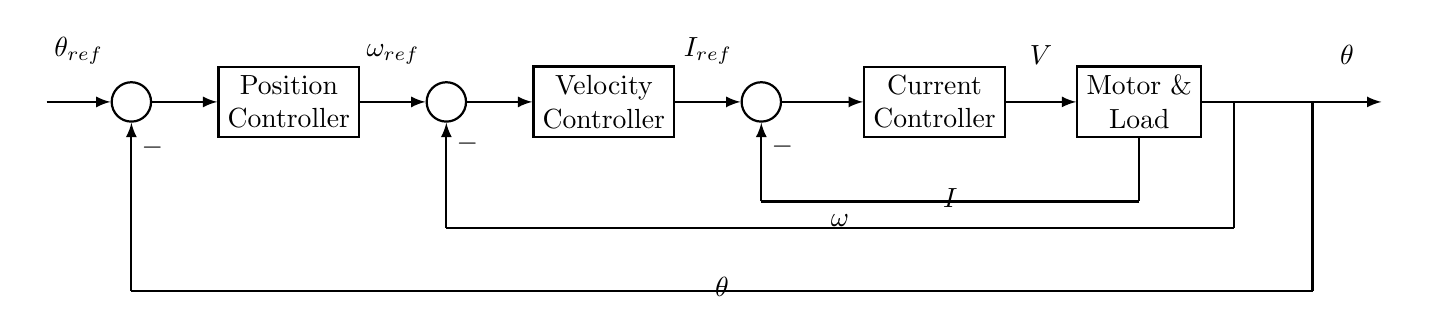
\begin{tikzpicture}[auto, >=latex]
        % تعريف الأنماط
        \tikzstyle{block} = [draw, rectangle, minimum height=2.5em, minimum width=3em, align=center, thick]
        \tikzstyle{sum} = [draw, circle, inner sep=0pt, minimum size=0.5cm, thick]
        
        \node (ref_pos) {};
        \node [sum, right of=ref_pos, node distance=1.2cm] (sum_pos) {};
        \node [block, right of=sum_pos, node distance=2cm] (ctrl_pos) {\textenglish{Position}\\\textenglish{Controller}};
        
        \node [sum, right of=ctrl_pos, node distance=2cm] (sum_vel) {};
        \node [block, right of=sum_vel, node distance=2cm] (ctrl_vel) {\textenglish{Velocity}\\\textenglish{Controller}};
        
        \node [sum, right of=ctrl_vel, node distance=2cm] (sum_cur) {};
        \node [block, right of=sum_cur, node distance=2.2cm] (ctrl_cur) {\textenglish{Current}\\\textenglish{Controller}};
        
        \node [block, right of=ctrl_cur, node distance=2.6cm] (motor) {\textenglish{Motor \&}\\\textenglish{Load}};
        
        % نقاط التفرع
        \coordinate [right of=motor, node distance=1.2cm] (takeoff_vel);
        \coordinate [right of=takeoff_vel, node distance=1cm] (takeoff_pos);
        \node [right of=takeoff_pos, node distance=1cm] (out_pos) {};

        % المسارات الأمامية مع إزاحة المتغيرات للأعلى
        \draw [->, thick] (ref_pos) -- node[midway, yshift=0.35cm] {$\theta_{ref}$} (sum_pos);
        \draw [->, thick] (sum_pos) -- (ctrl_pos);
        \draw [->, thick] (ctrl_pos) -- node[midway, yshift=0.35cm] {$\omega_{ref}$} (sum_vel);
        \draw [->, thick] (sum_vel) -- (ctrl_vel);
        \draw [->, thick] (ctrl_vel) -- node[midway, yshift=0.35cm] {$I_{ref}$} (sum_cur);
        \draw [->, thick] (sum_cur) -- (ctrl_cur);
        \draw [->, thick] (ctrl_cur) -- node[midway, yshift=0.35cm] {$V$} (motor);
        
        % خط الخرج
        \draw [-, thick] (motor) -- (takeoff_vel);
        \draw [-, thick] (takeoff_vel) -- (takeoff_pos);
        \draw [->, thick] (takeoff_pos) -- node[midway, yshift=0.35cm] {$\theta$} (out_pos);

        % التغذية الراجعة للتيار
        \draw [thick] (motor.south) -- ++(0,-0.8) coordinate (fb_I);
        \draw [thick] (fb_I) -- node[midway, yshift=0.3cm] {$I$} (fb_I -| sum_cur.south);
        \draw [->, thick] (fb_I -| sum_cur.south) -- node[pos=0.7, right] {$-$} (sum_cur.south);
        
        % التغذية الراجعة للسرعة
        \draw [thick] (takeoff_vel) -- ++(0,-1.6) coordinate (fb_w);
        \draw [thick] (fb_w) -- node[midway, yshift=0.3cm] {$\omega$} (fb_w -| sum_vel.south);
        \draw [->, thick] (fb_w -| sum_vel.south) -- node[pos=0.8, right] {$-$} (sum_vel.south);
        
        % التغذية الراجعة للموقع
        \draw [thick] (takeoff_pos) -- ++(0,-2.4) coordinate (fb_t);
        \draw [thick] (fb_t) -- node[midway, yshift=0.3cm] {$\theta$} (fb_t -| sum_pos.south);
        \draw [->, thick] (fb_t -| sum_pos.south) -- node[pos=0.85, right] {$-$} (sum_pos.south);

    \end{tikzpicture}%
    }
    \caption[المخطط الصندوقي لهيكلية حلقات التحكم المتداخلة في أنظمة السيرفو]{\centering المخطط الصندوقي لهيكلية حلقات التحكم المتداخلة في أنظمة السيرفو}
    \label{fig:cascaded_loops}
\end{figure}

\subsection{الحلقة الداخلية: حلقة التيار/العزم (\textenglish{Current/Torque Loop})}
تُعد حلقة التحكم في التيار هي خط الدفاع الأول والأسرع استجابة. تقع هذه الحلقة فعلياً داخل مشغل السيرفو (\textenglish{Servo Drive})، والهدف الأساسي منها هو التحكم الدقيق في التيار المار عبر ملفات العضو الثابت لإجبار المحرك على إنتاج العزم الميكانيكي المطلوب $T_{ref}$.

تُحكم الديناميكا الكهربائية بالمعادلة التفاضلية التالية:
$$V(t) = R \cdot i(t) + L \frac{di(t)}{dt} + E_b(t)$$
وبما أن العزم الميكانيكي يتناسب طردياً مع التيار الفعال ($T = K_t \cdot i$)، فإن التحكم في التيار يعني فعلياً التحكم في العزم. نظراً لصغر الثابت الزمني الكهربائي $\tau_e = L/R$، يُستخدم متحكم تناسبي-تكاملي (\textenglish{PI}) بترددات أخذ عينات عالية جداً تصل إلى عشرات الكيلوهرتز للتعامل مع التغيرات اللحظية وتقليل خطأ التيار إلى الصفر.

\subsection{الحلقة الوسطى: حلقة السرعة (\textenglish{Velocity Loop})}
وظيفتها الأساسية هي مقارنة السرعة المطلوبة $\omega_{ref}$ (القادمة من مخرج حلقة الموقع) مع السرعة الفعلية $\omega$ (المقاسة بواسطة المشفر)، ومن ثم توليد إشارة مرجعية للتيار $I_{ref}$ للحلقة الداخلية.

نظراً لأن الأنظمة الميكانيكية تتعرض باستمرار للاحتكاك واضطرابات التحميل الخارجية، يُستخدم بشكل شبه دائم متحكم تناسبي-تكاملي (\textenglish{PI}) في هذه الحلقة:
\begin{itemize}
    \item \textbf{الجزء التناسبي (\textenglish{P}):} يوفر استجابة فورية لأخطاء السرعة اللحظية.
    \item \textbf{الجزء التكاملي (\textenglish{I}):} يضمن القضاء التام على خطأ الحالة المستقرة عند تطبيق عزم حمل ثابت على المحرك.
\end{itemize}

\subsection{الحلقة الخارجية: حلقة الموقع (\textenglish{Position Loop})}
هي الحلقة الأبطأ من حيث سرعة الاستجابة. تستقبل مسار الحركة المطلوب $\theta_{ref}$، وتقارنه بالموقع الزاوي الفعلي $\theta$، لتُصدر السرعة المطلوبة $\omega_{ref}$ للحلقة الوسطى.

على عكس حلقة السرعة، يُكتفى عادةً باستخدام متحكم \textbf{تناسبي فقط (\textenglish{P Controller})} في حلقة الموقع. ويعود السبب الرياضي في ذلك إلى العلاقة التكاملية بين السرعة والموقع:
$$\theta(t) = \int_{0}^{t} \omega(\tau) d\tau$$
النظام الميكانيكي يمتلك بطبيعته "مُكاملاً طبيعياً" ($1/s$). لذلك، إضافة جزء تكاملي إضافي سيؤدي إلى تقليل هامش الاستقرار والتسبب باهتزاز المحرك وتجاوز الهدف (\textenglish{Overshoot}).